\documentclass[11pt]{article}

%defines page size and margins
\usepackage{geometry}
\geometry{
  letterpaper,
  left=1in,
  right=1in,
  top=1in,
  bottom=1in,
}

%Sets spacing for entire document
\usepackage{setspace}
\singlespacing

%Package for reducing space in between list items
\usepackage{enumitem}

%Links
\usepackage{hyperref}

%Math symbols
\usepackage{gensymb}

%For floating images
\usepackage{caption}
\usepackage{float}

%better tables
\usepackage{multirow}
\usepackage{array}

\usepackage{longtable}

%Used for adjusting images
\usepackage[export]{adjustbox}

%Image path
\usepackage{graphicx}
\usepackage{animate}

\begin{document}

{\Large\noindent Brett Levenson, Andy Poulos, Rishabh Shah, John Stefan

\noindent October 31, 2017

\noindent Lab 3 \\}

\section*{Exercise One}
\begin{figure}[H]
	\centering
	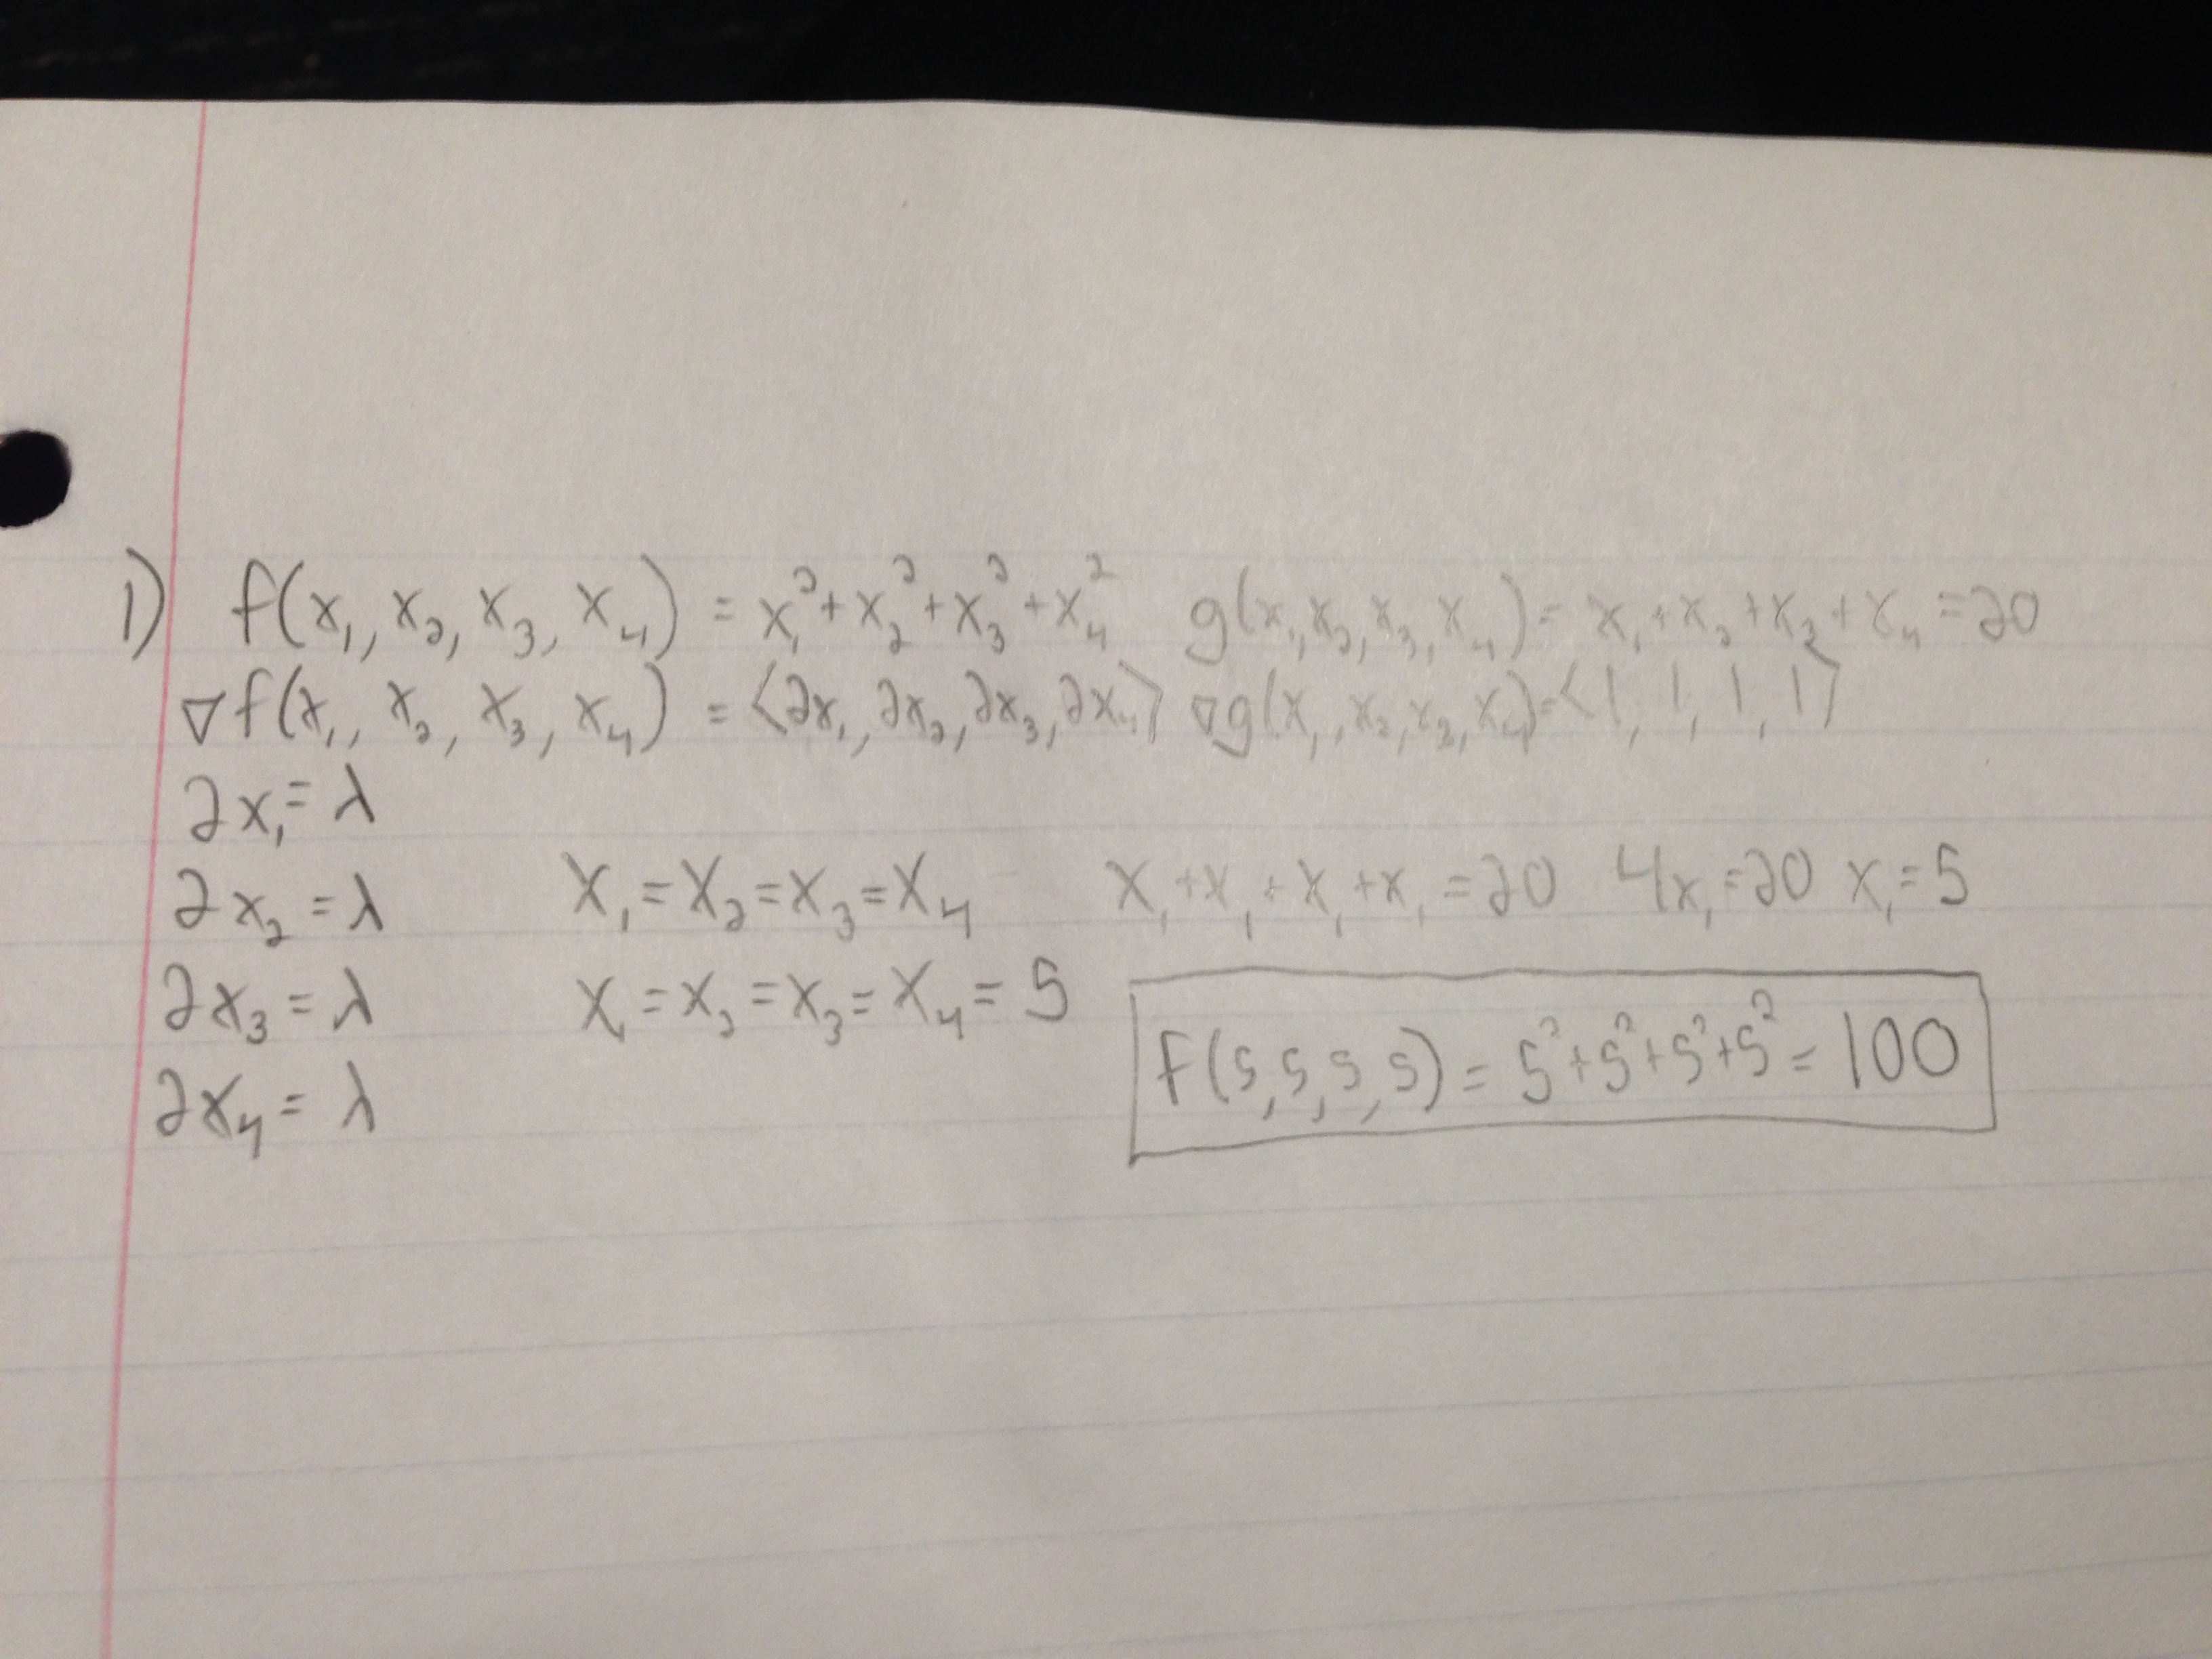
\includegraphics[width=\textwidth]{One.JPG}
\end{figure}

\section*{Exercise Two}
\begin{figure}[H]
	\centering
	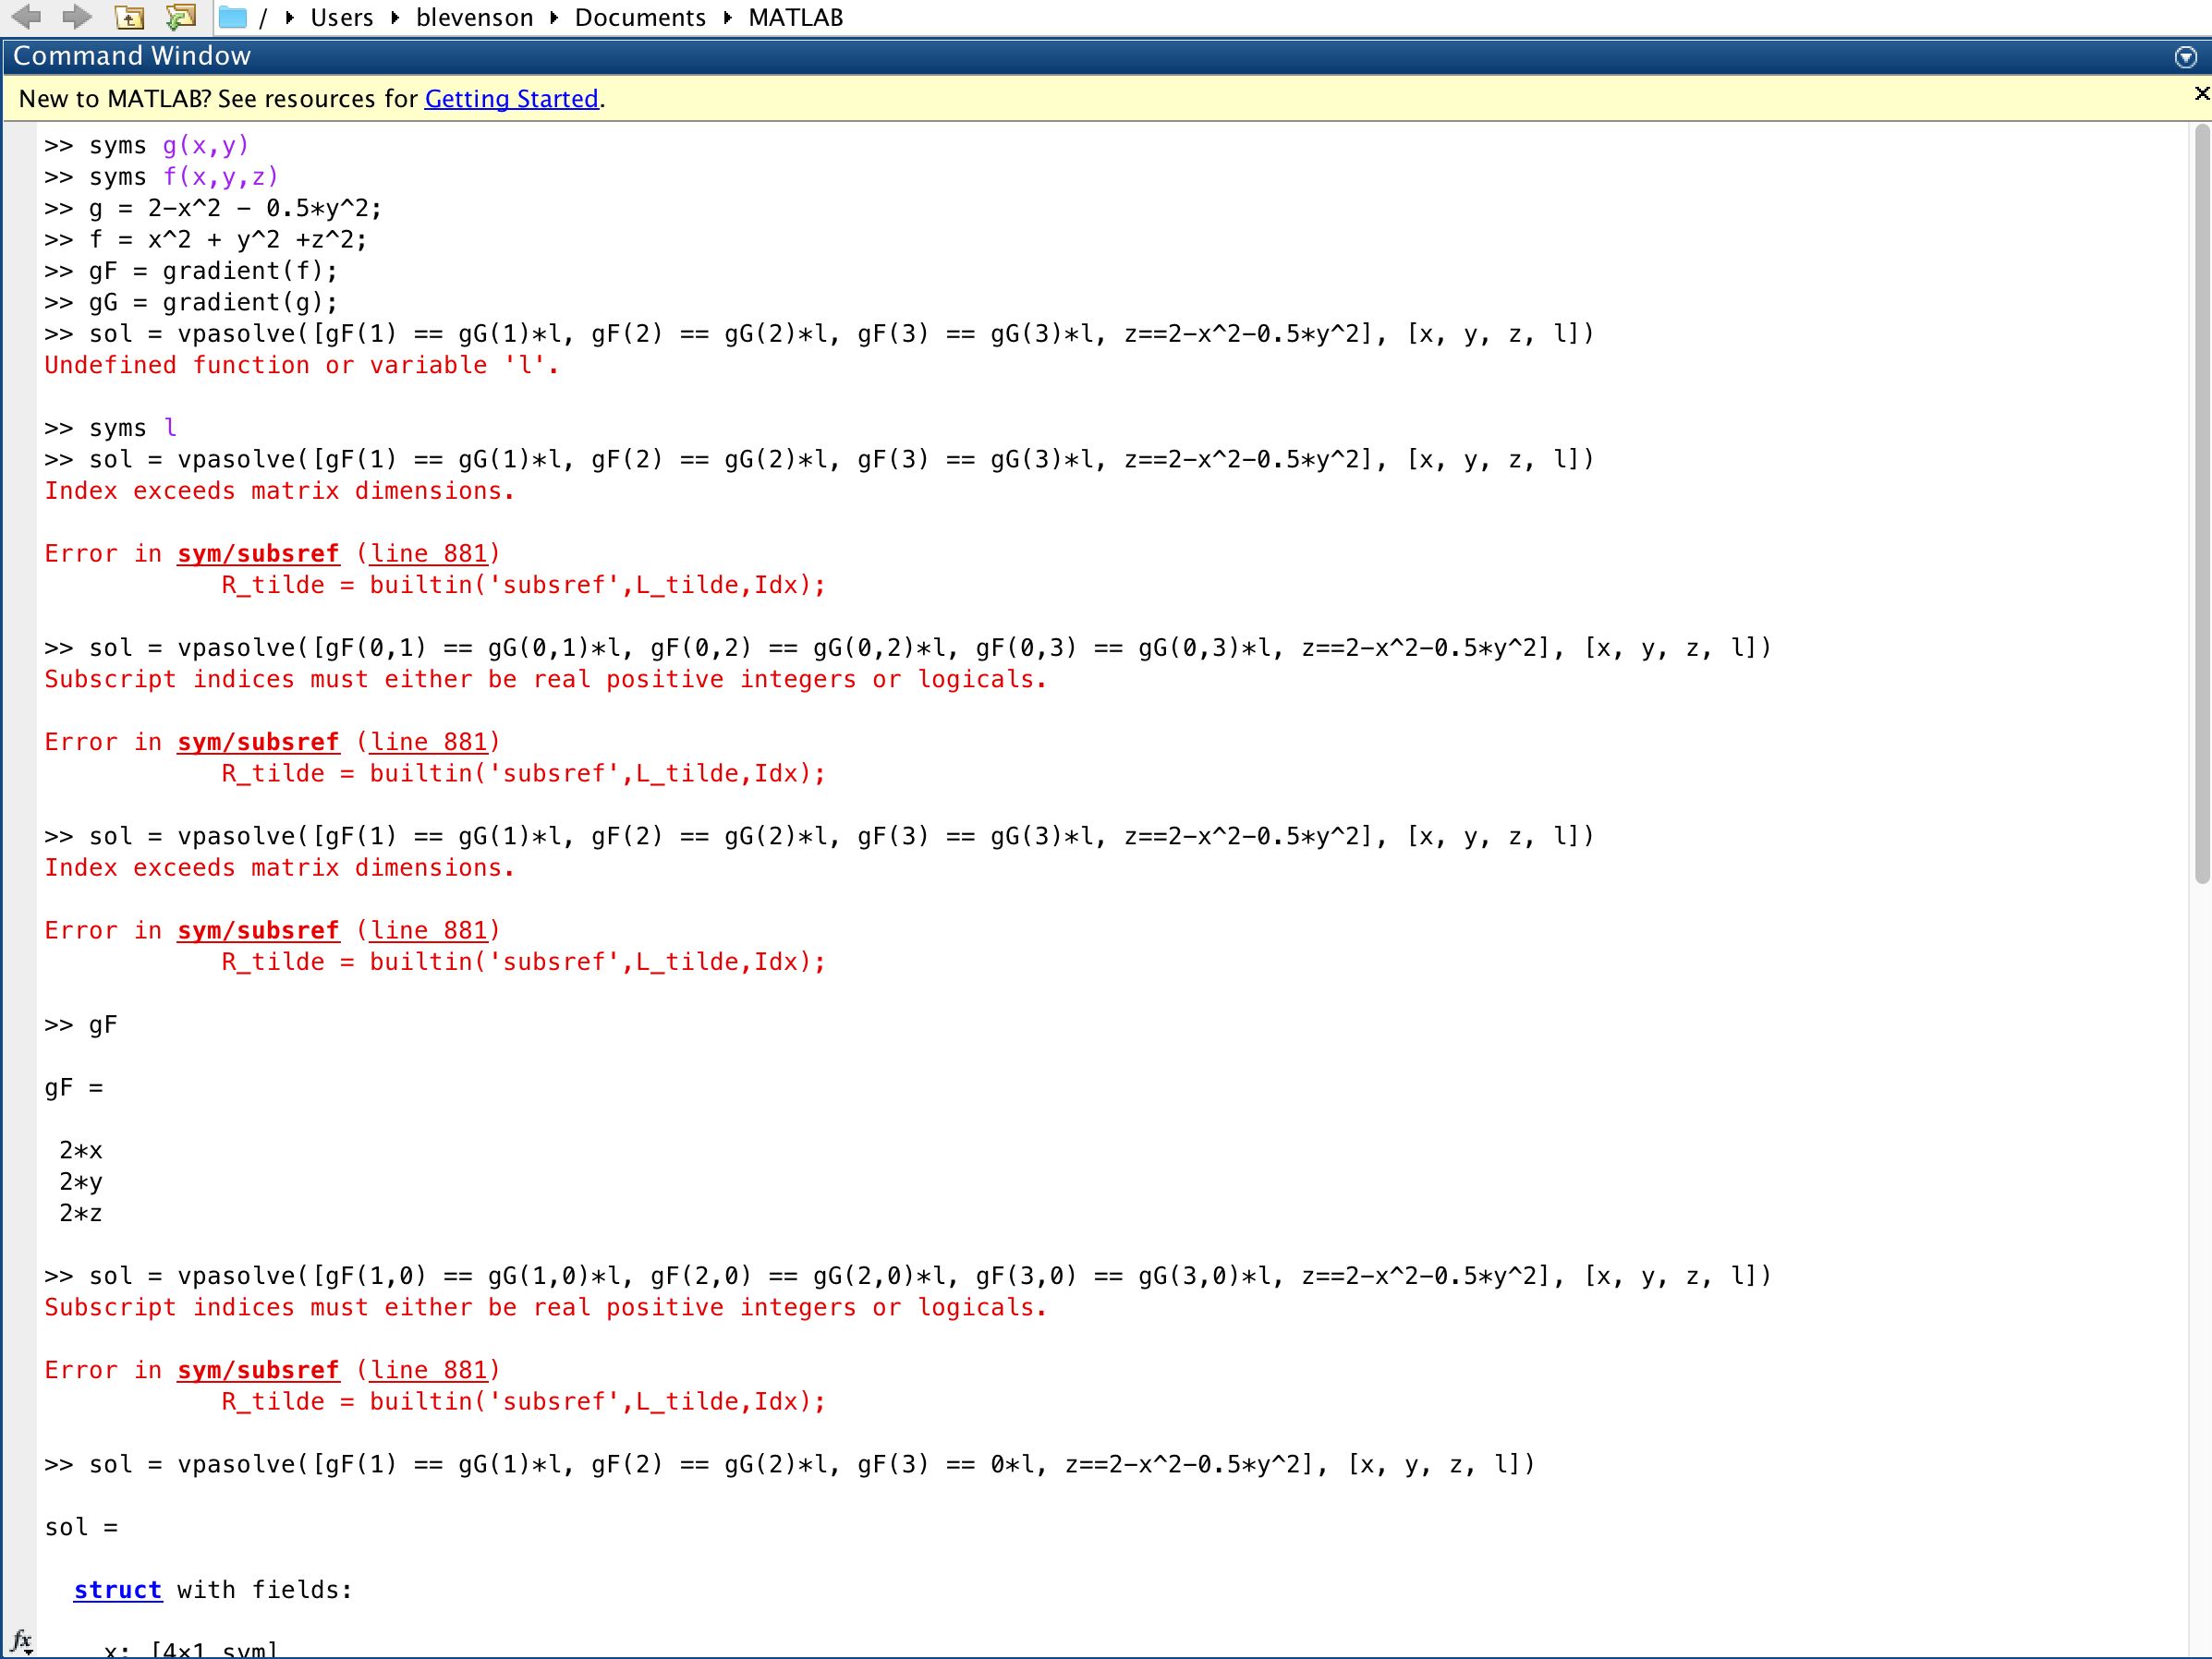
\includegraphics[width=\textwidth]{Prob2PartA.png}
\end{figure}
\begin{figure}[H]
	\centering
	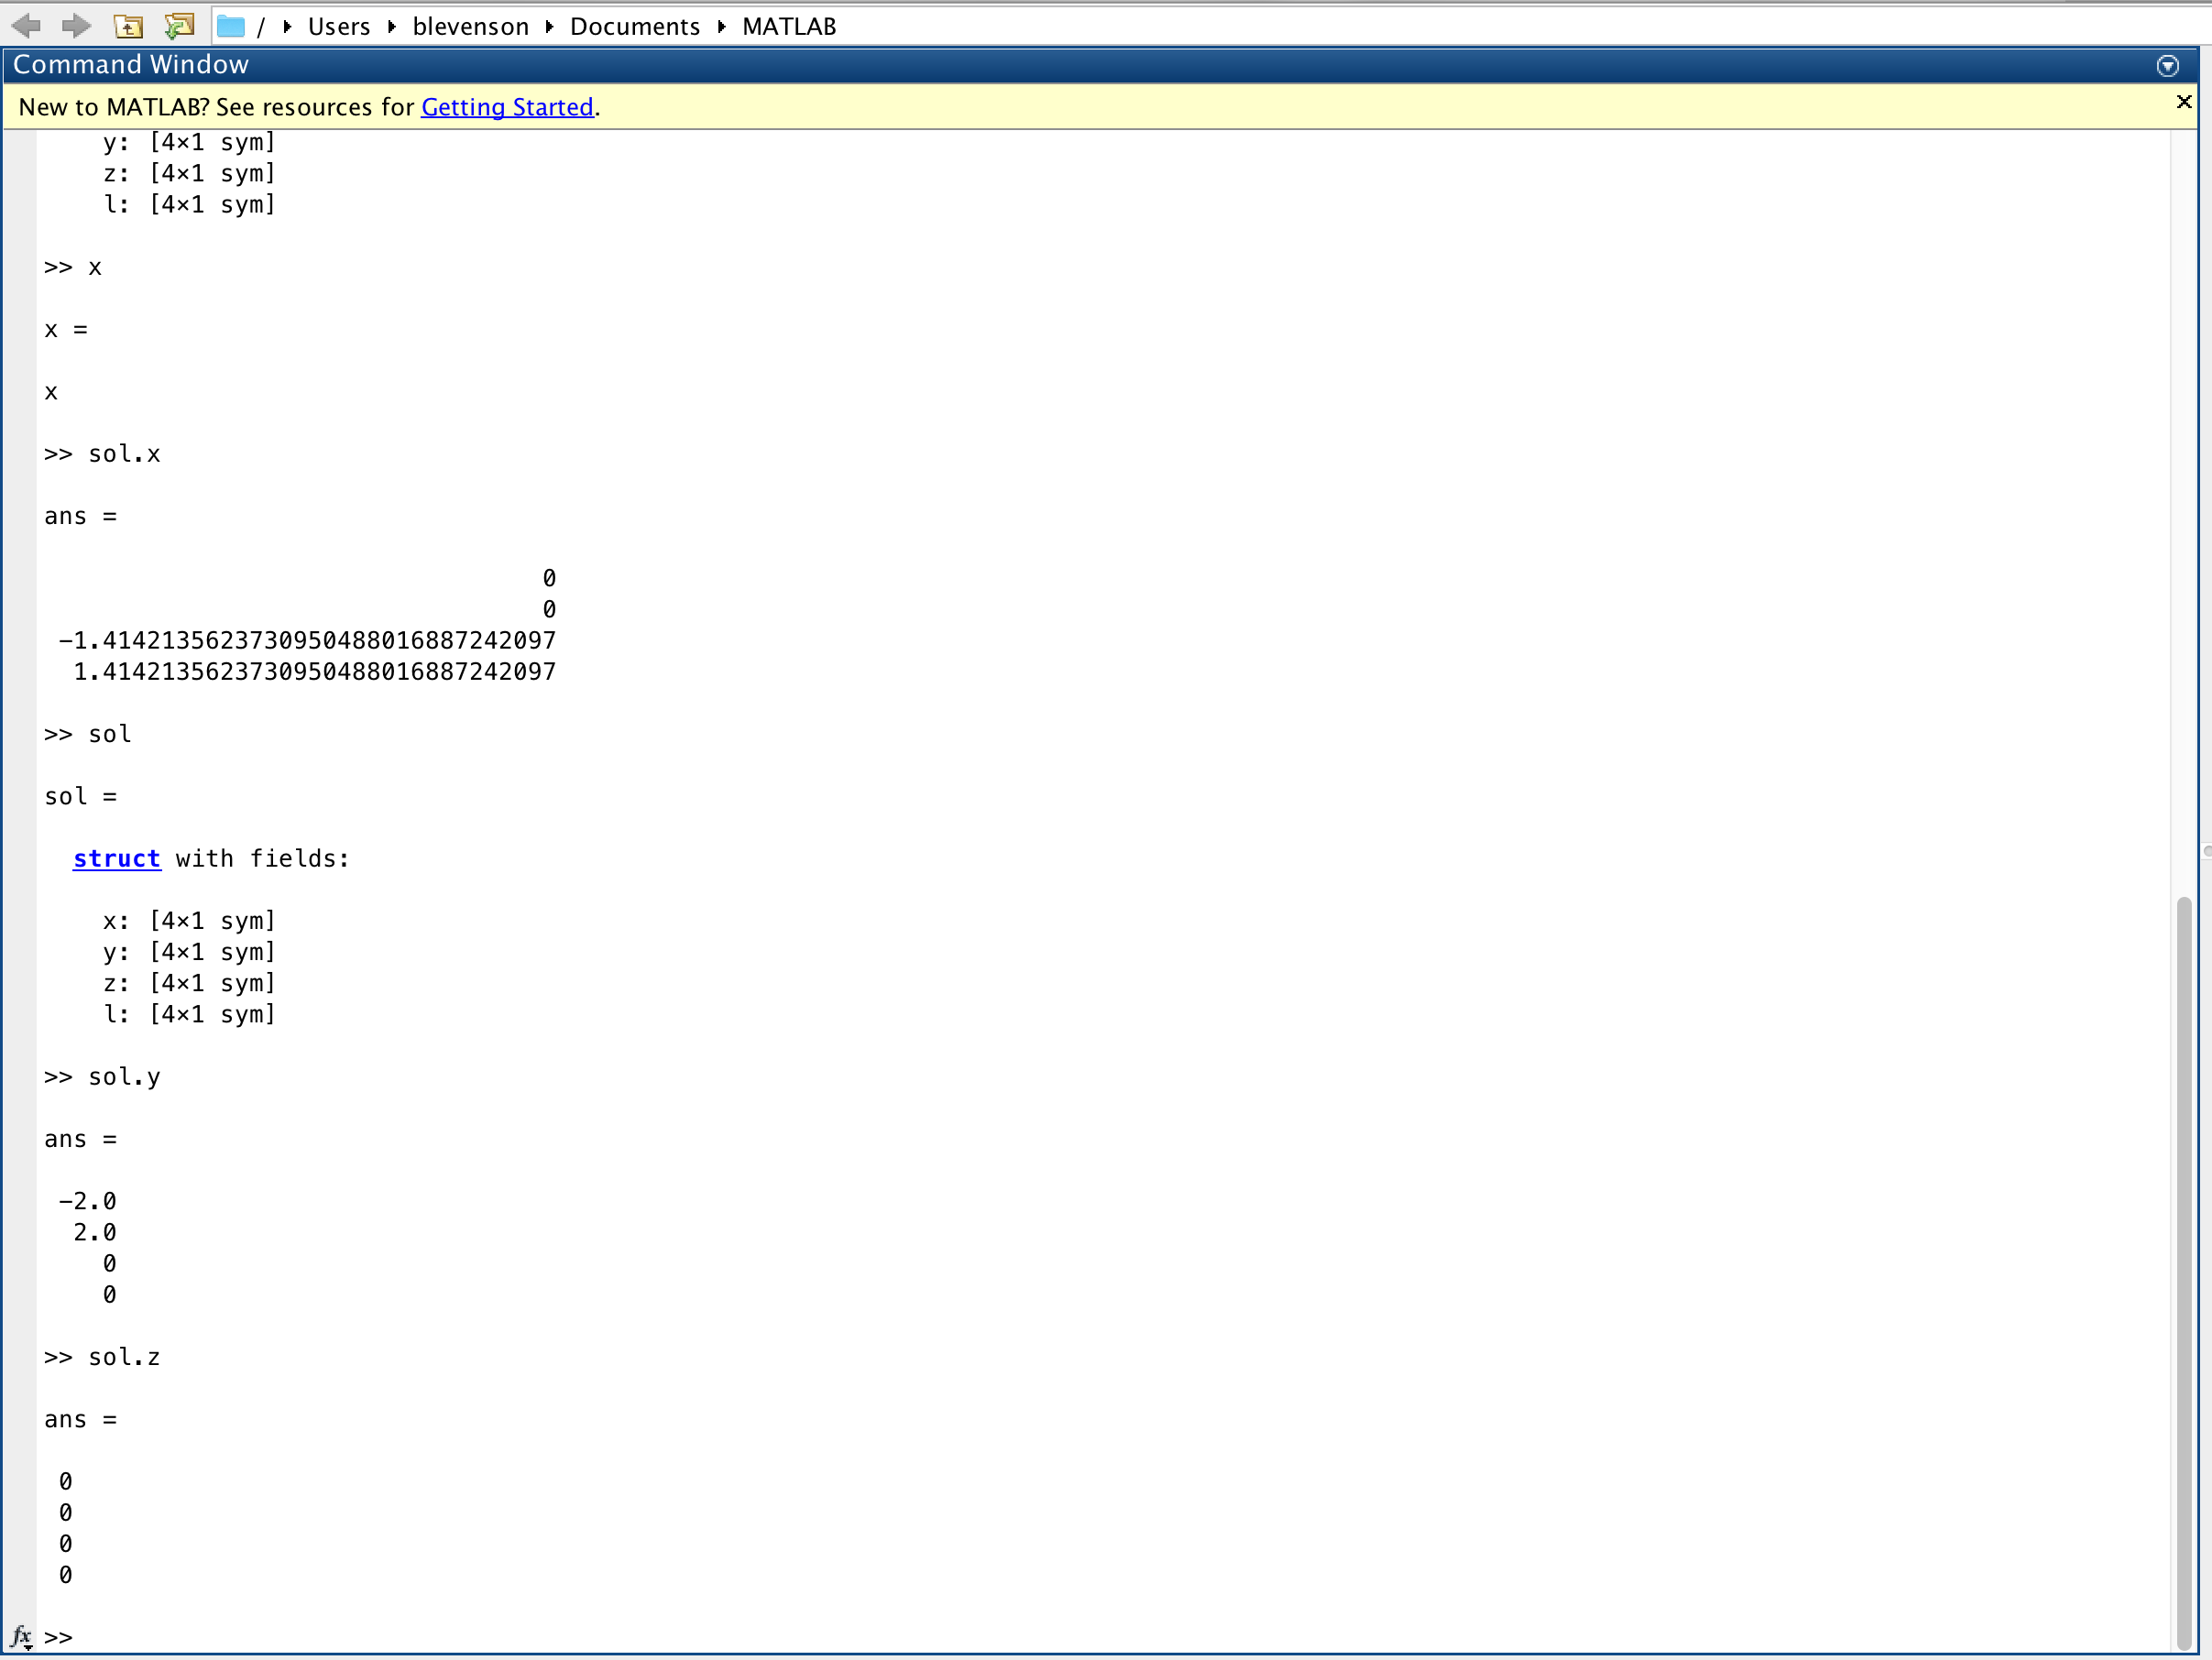
\includegraphics[width=\textwidth]{Prob2PartB.png}
	\caption*{The solutions that work are: $(0, -2, 0), (0,0,0), (-1.4142, -2, 0), (-1.4142, 0, 0), (1.4142, -2, 0)$.}
\end{figure}

\section*{Exercise Three}
\begin{figure}[H]
	\centering
	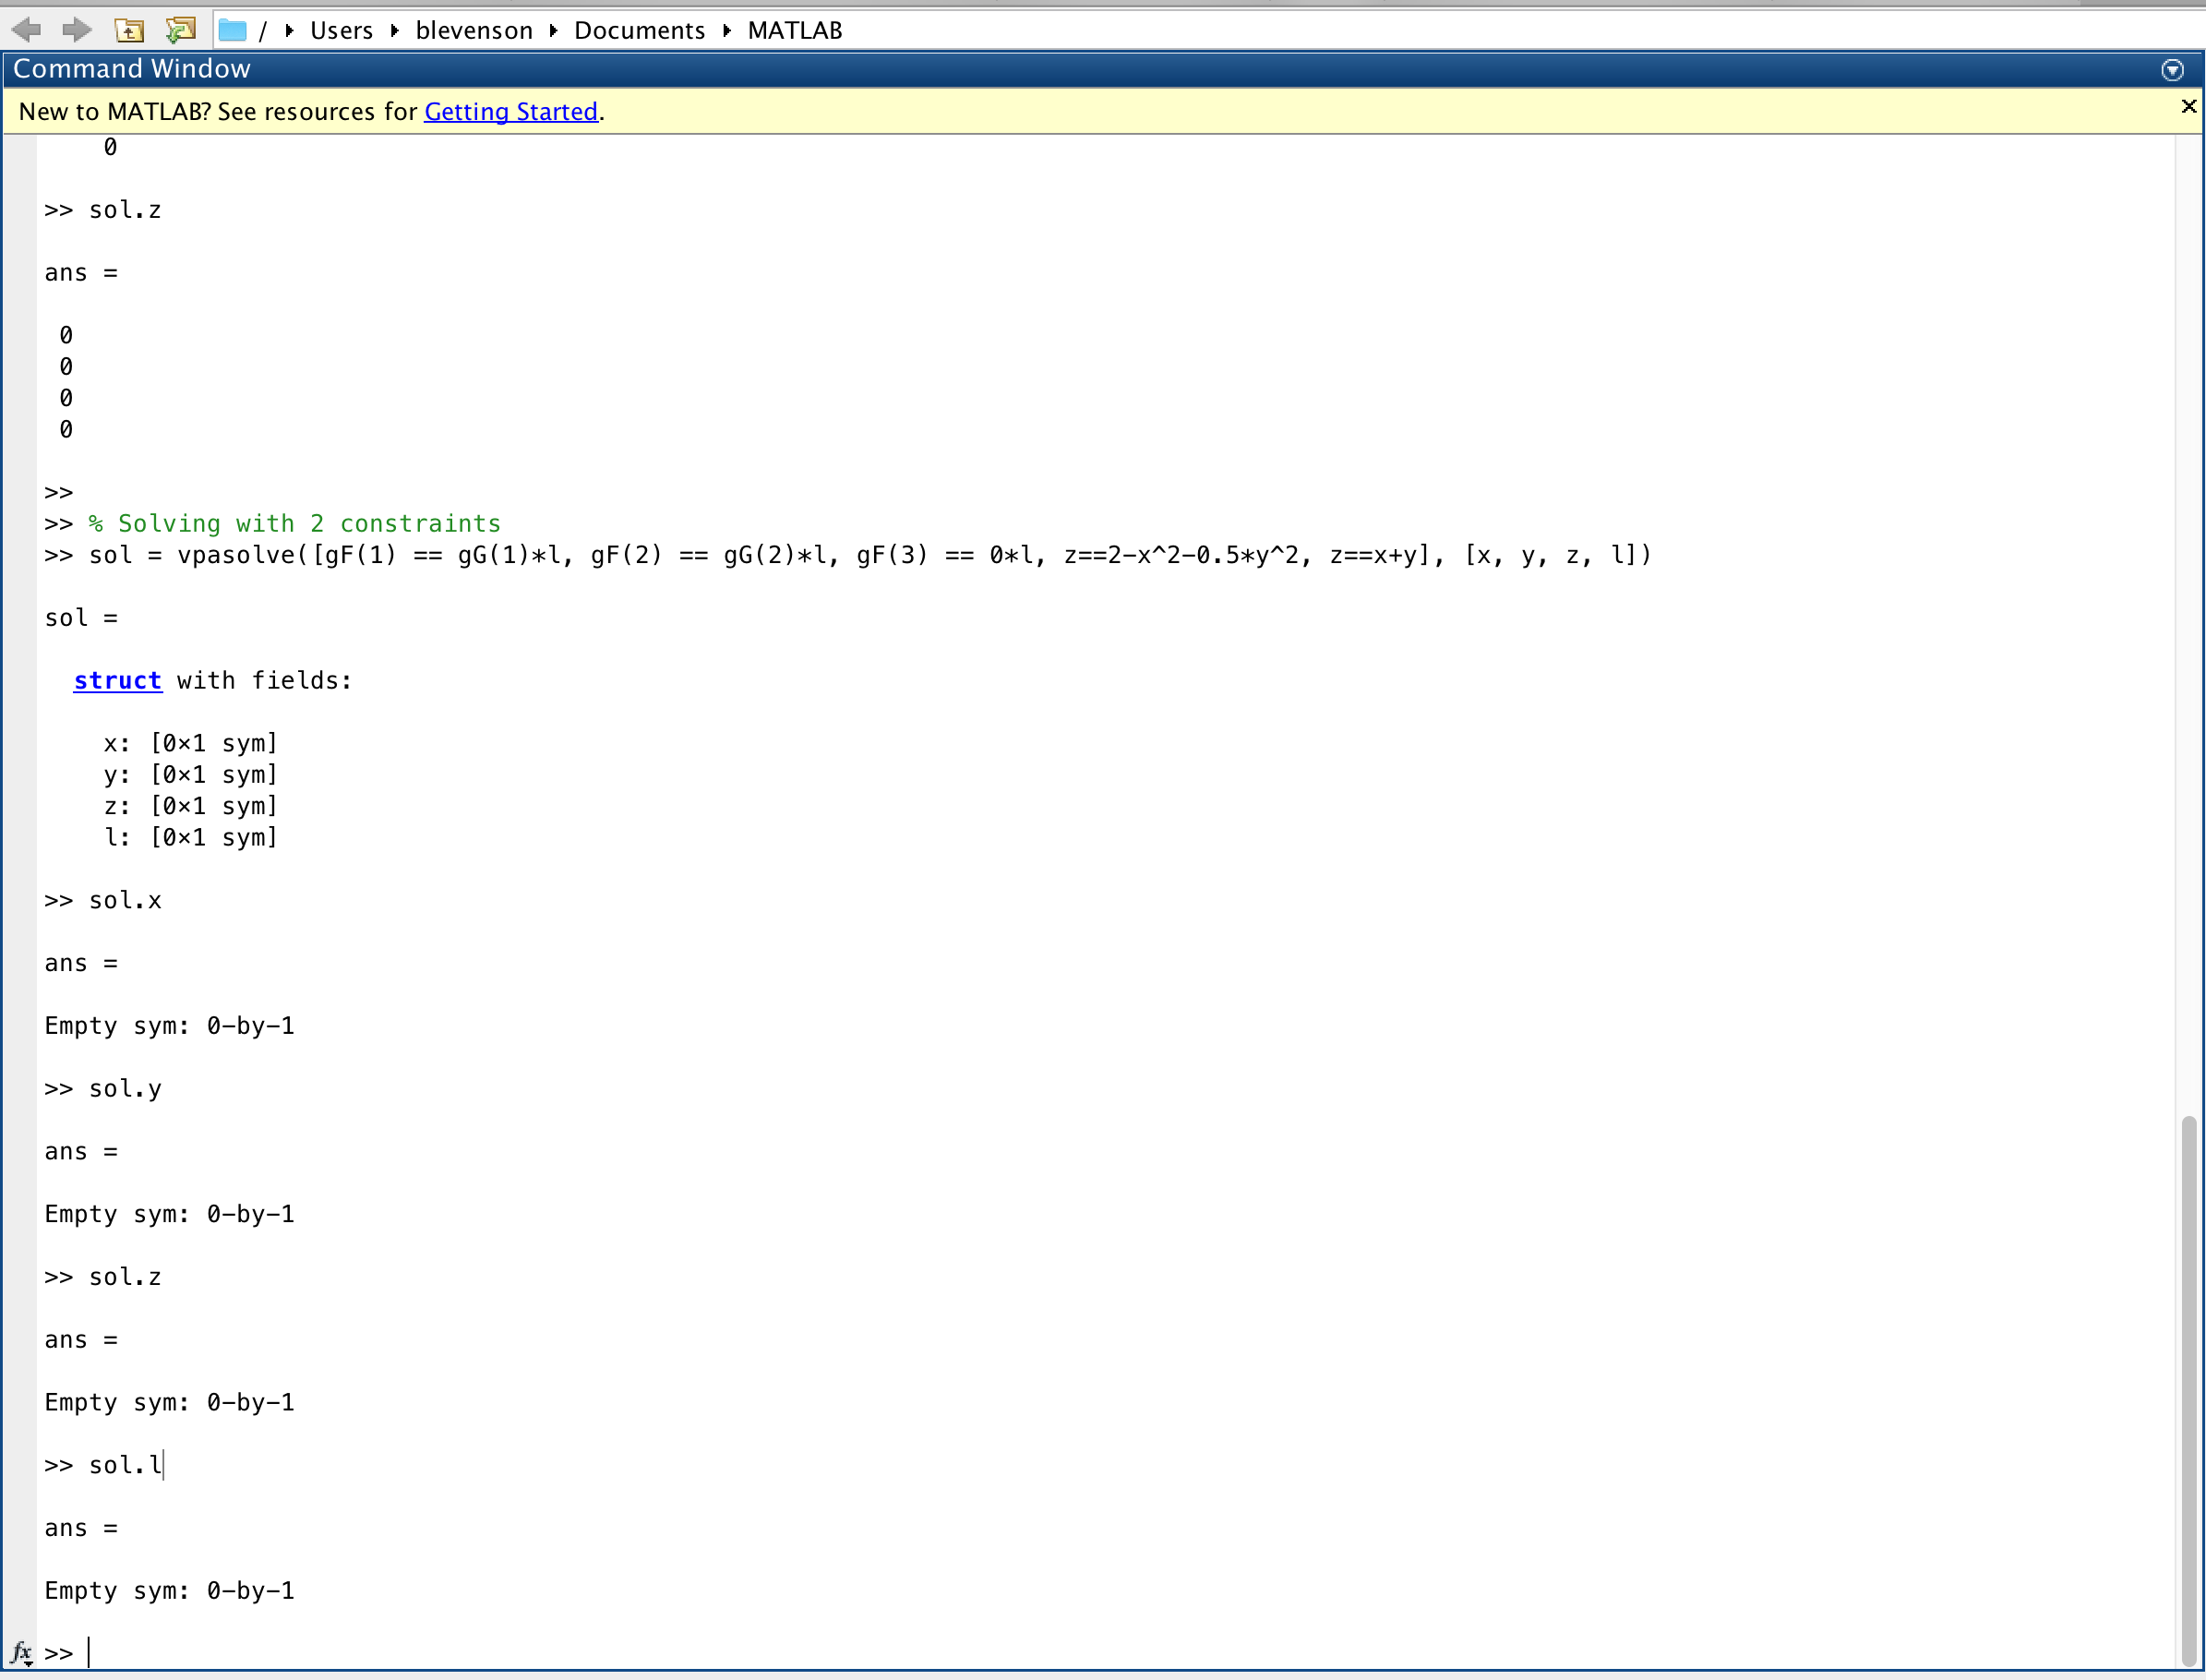
\includegraphics[width=\textwidth]{Prob3.png}
	\caption*{When solving the system with two constraints, there are no critical points of $f(x, y, z)$ constrained by the boundary. This is because the space has been overrefined, preventing any points from fulfilling both the constraints and the LaGrange multiplier equations. Because there are no points in the boundary, we are unable to determine if the gradients are linearly independent at every point on the boundary.}
\end{figure}

\section*{Exercise Four}
\begin{figure}[H]
	\centering
	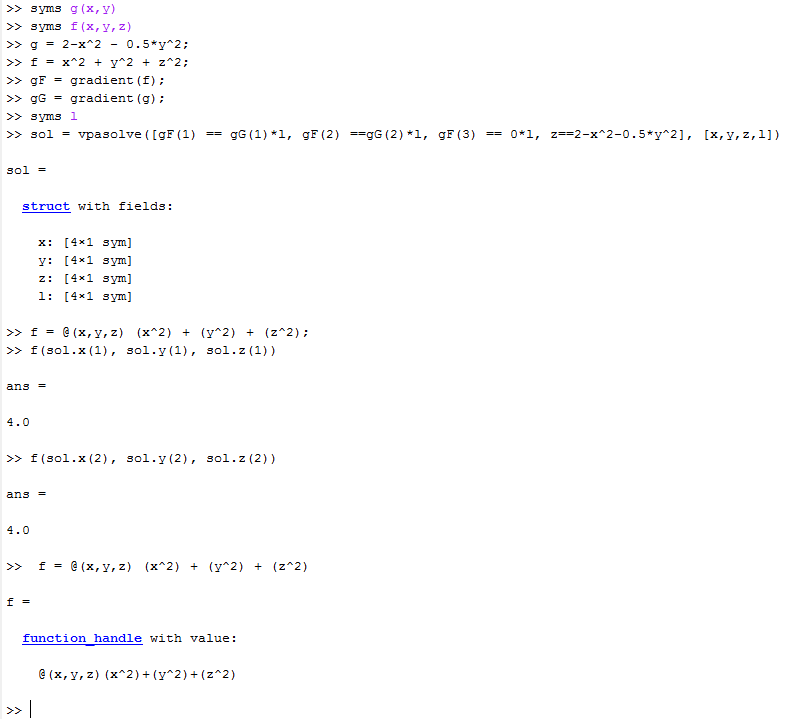
\includegraphics[width=\textwidth]{Four.PNG}
	\caption*{The maximum value is $4.0$ from the point $(0, 0, 2)$ and the minimum is $1.75$ from the point $(-1.2247, 0, 0.5)$.}
\end{figure}

\section*{Exercise Five}
\begin{figure}[H]
	\centering
	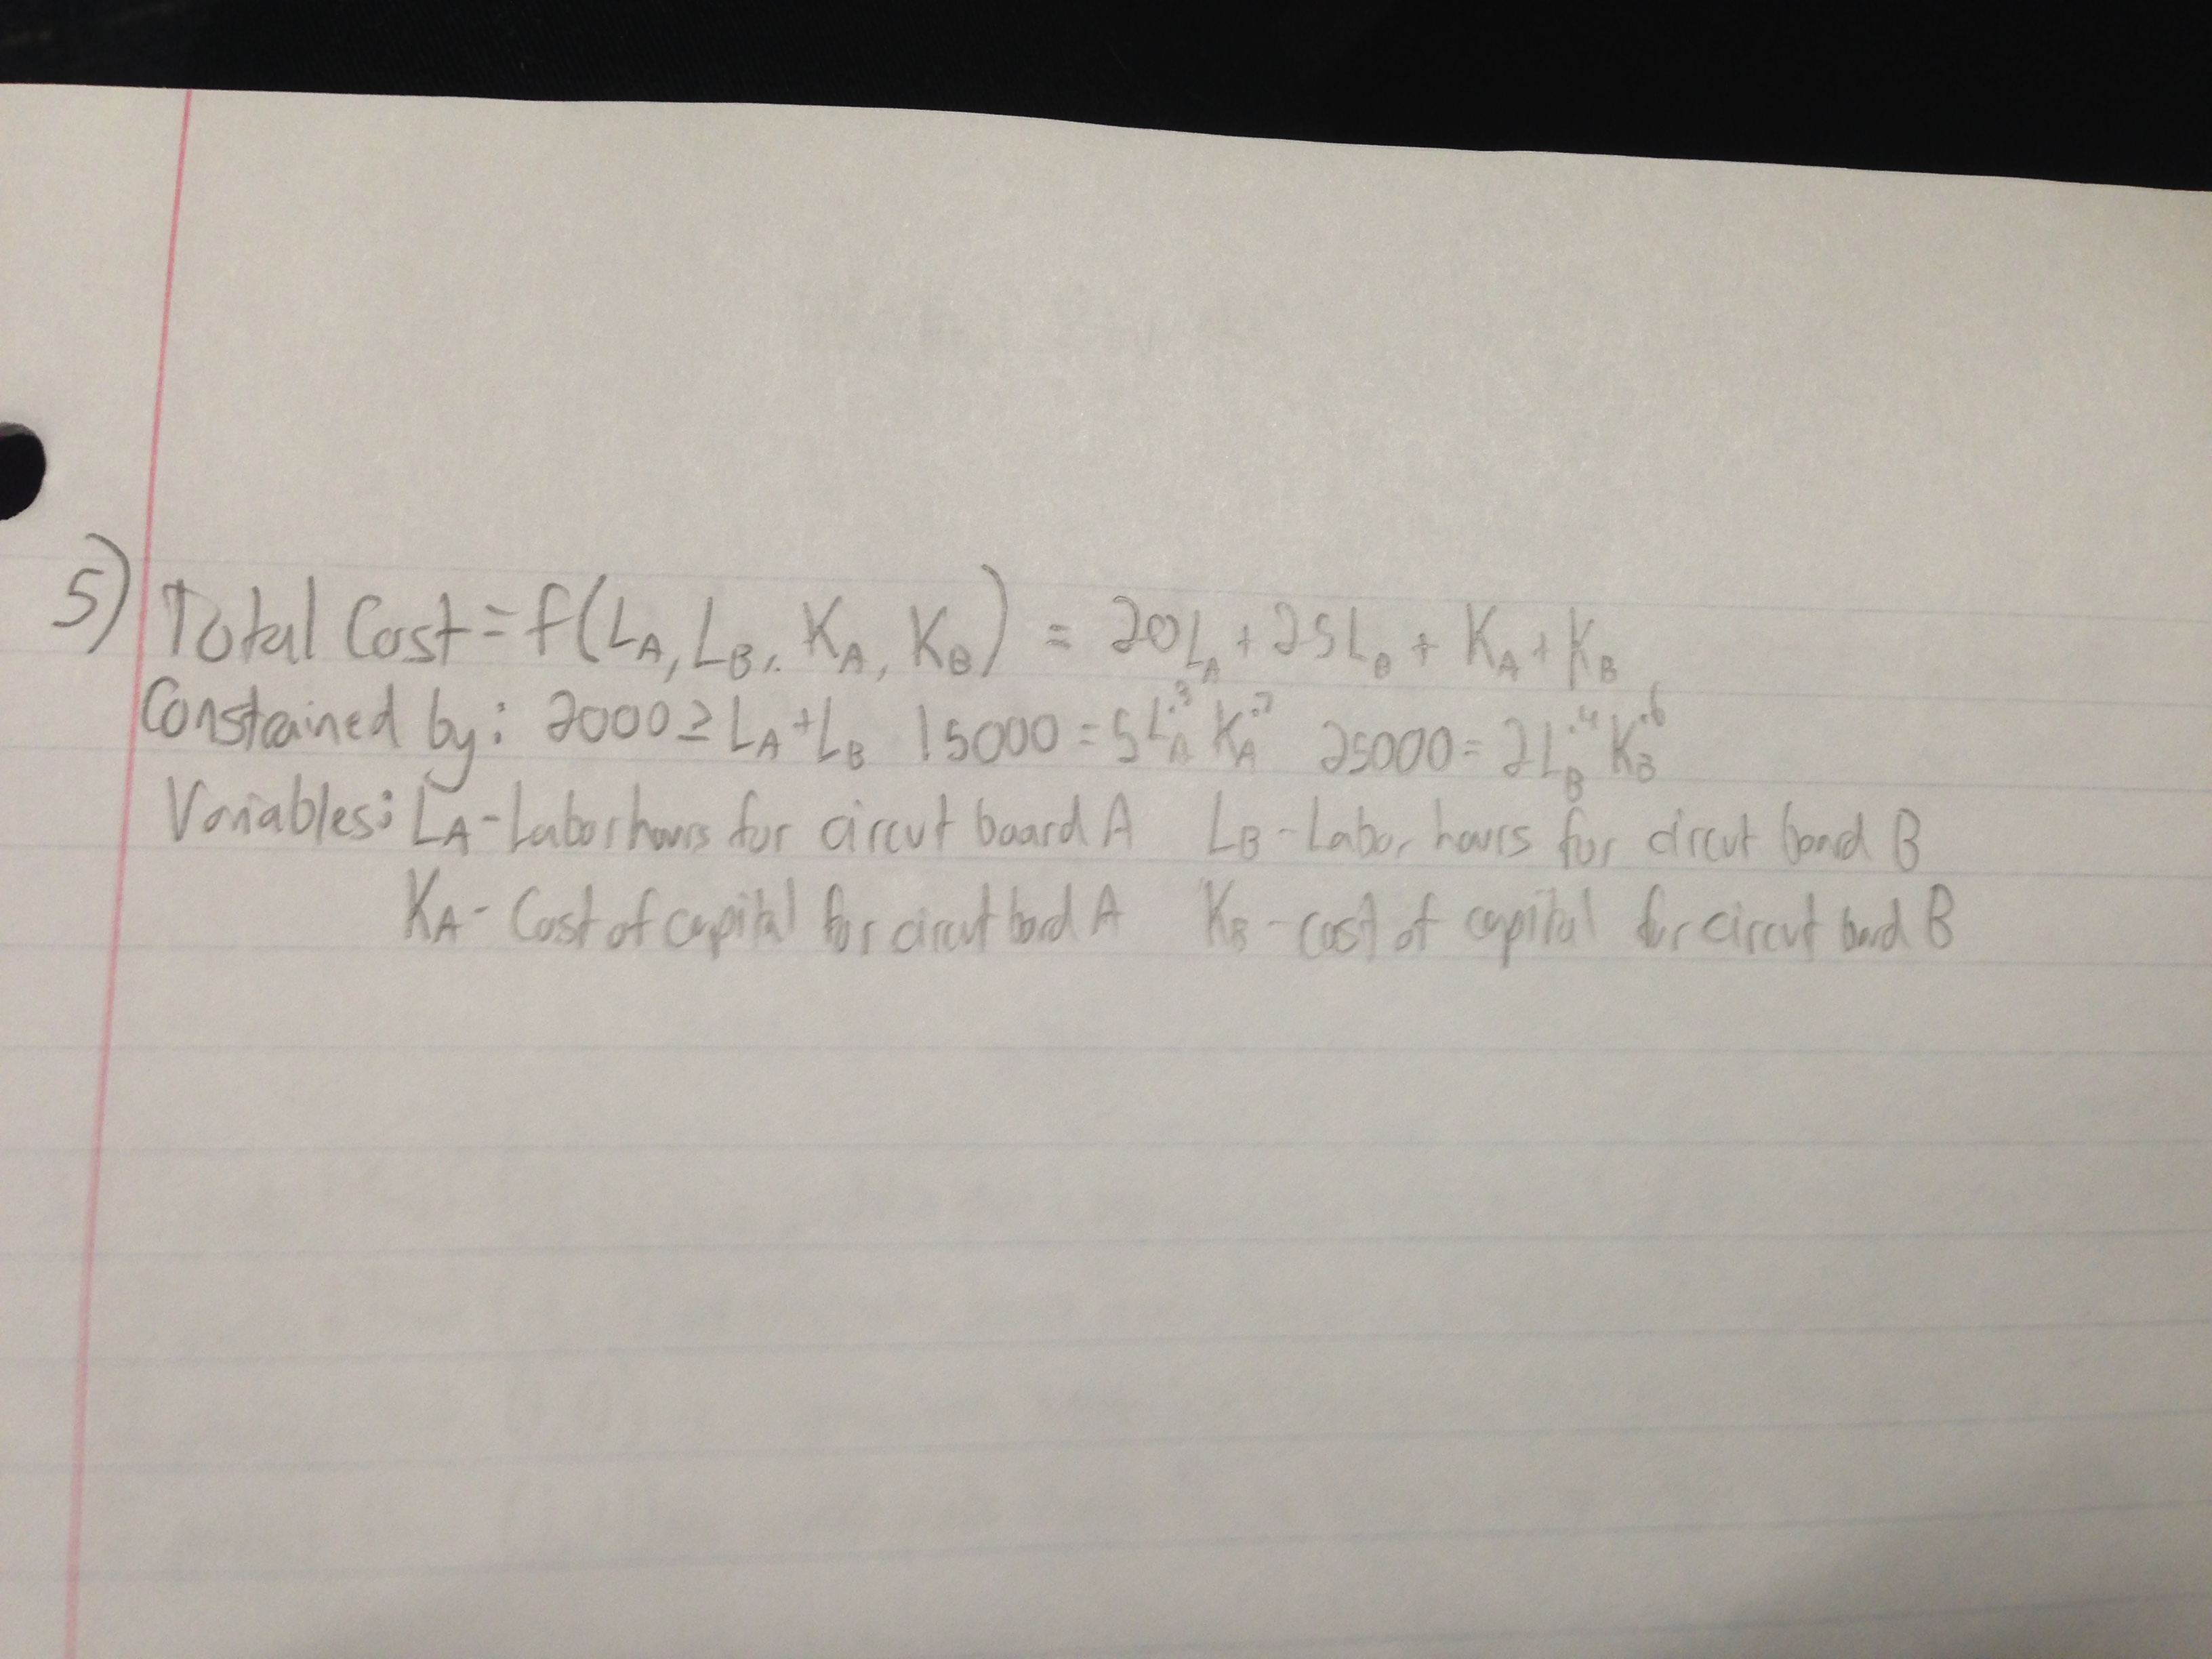
\includegraphics[width=\textwidth]{Five.JPG}
\end{figure}

\section*{Exercise Six}
\begin{figure}[H]
	\centering
	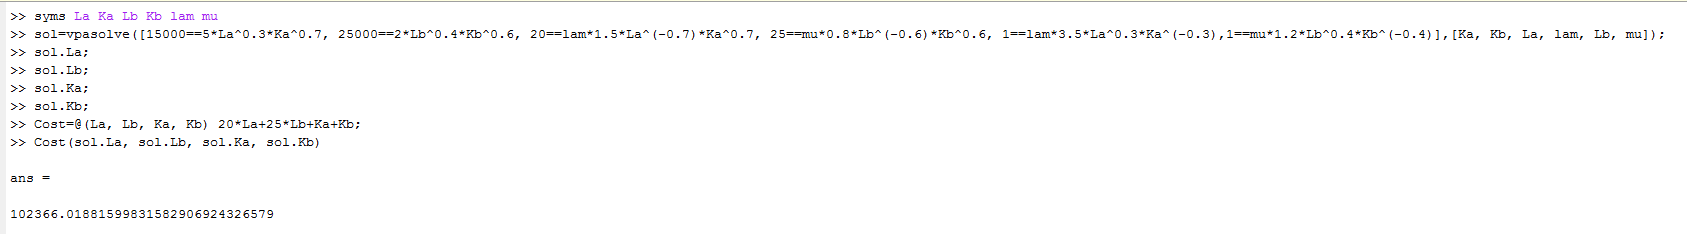
\includegraphics[width=\textwidth]{Six.PNG}
	\caption*{Running the function gave the critical point $(203.62, 1420.7, 9502.2, 53275)$, returning a total cost of \$102,366.02.}
\end{figure}

\section*{Exercise Seven}
\begin{figure}[H]
	\centering
	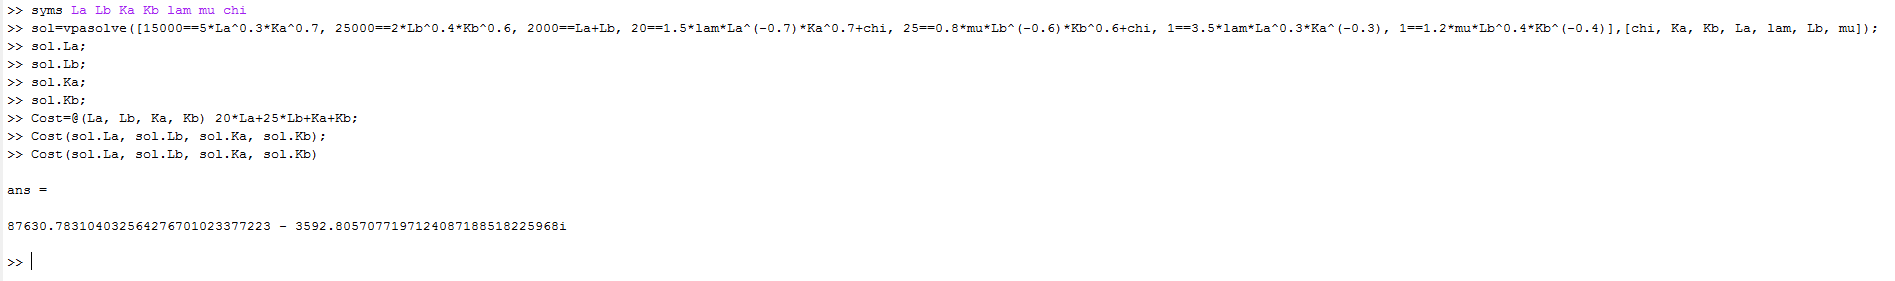
\includegraphics[width=\textwidth]{Seven.PNG}
	\caption*{Running the function returns a critical point consisting of imaginary numbers, meaning there are no critical points on the boundary constraint $La+Lb=2000$. Therefore the minimum cost is the cost found in Exercise 6, \$102,366.02.}
\end{figure}

\end{document}